\Section{MPEG Decoder in StreamIt}

% TODO: recalculate lines of code using statement count (num of ;)
We implemented an MPEG-2 decoder in StreamIt. It is a fully portable
implementation in that the application is not architecture
dependent. The implementation was carried out by one student
programmer with no prior understanding of MPEG. The development
spanned eight weeks from specification~\cite{MPEG2} to the first fully
functional MPEG decoder. The StreamIt code is nearly 4,921 lines of
code with 48 static streams. The MPEG stream parser is the largest
single filter, consisting of 1,924 lines of code.  The 48 static
streams are compiled to 2,150 filters for a picture resolution of
352x240. In contrast, the reference C
implementation~\cite{reference-mpeg-c} is nearly 9,832 lines of code,
although it provides several features such as interlacing and
multi-layer streams that are not yet implemented in the StreamIt
decoder.

A noteworthy aspect of the StreamIt implementation is its
malleability. We illustrate this using two specific examples. 
In the first example, we focus on the video sampling rates. MPEG-2
streams are encoded using a 4:2:0 sampling rate, which achieve a 50\%
reduction in the number of bits required to represent a video, with
little noticeable loss of color. However, better quality is possible
with higher sampling rates since more color information is retained
from the original picture. In this paper, we describe how our
decoder implementation, originally designed to deal with 4:2:0
sampling rate is modified for a 4:2:2 sampling rate.

In the second example, we describe a straight forward language-level
transformation that exposes the data-parellism across macroblocks in a
picture. This is done in the context of the decoder pipeline which
consits of the inverse quantization, inverse DCT, and motion
compensator. We decribe parallelism can be exposed at various levels
in the decoding process, from macroblock to block granularities. We
show that the migration path is trivial.

\SubSection{Video Sampling Rate}

Macroblocks specify colors using a luminance channel to represent
saturation (color intensity), and two chrominance channels to
represent hue. The human eye is more sensitive to changes in
saturation than changes in hue, so the chrominance channels are
frequently compressed by downsampling the chrominance data within a
macroblock. The type of chrominance downsampling an MPEG-2 encoder
uses is its {\it chrominance format}. The most common chrominance
format is 4:2:0, which uses a single block for each of the chrominance
channels, downsampling each of the two channels from 16x16 to 8x8.  An
alternate chrominance format is 4:2:2. It uses two blocks for each
chrominance channel, downsampling each of the channels from 16x16 to
8x16. The possible chrominance formats are shown in
Figure~\ref{fig:chroma-format}.

To support the 4:2:2 chrominance format in our StreamIt decoder, we
modified 31 lines and added 20 new lines. Of the 31 modified lines, 23
were trivial modifications to pass a variable representing the
chrominance format as a stream parameter. The greatest substantial
change was to the decoding splitjoin previously illustrated in
Figure~\ref{fig:decoding-sj}. In the case of a 4:2:2 sampling rate,
the chrominance data, as it appears on the input tape, alternates
between each of the two chrominance channels. Thus, a a two-tiered
splitjoin is used to properly recover the appropriate chrominance
channels. The new splitjoin is shown in Figure~\ref{fig:chroma-format}.
\begin{figure*}[t]
 \begin{minipage}[t]{4.0in}
   {
    \begin{scriptsize}
    \begin{verbatim} 
    // N = macroblock size + motion vector data size;
    // W = picture width (resolution in pixels);
    // H = picture width (resolution in pixels);

    int->int splitjoin(int chromaFormat) {
      int xUpSample, yUpSample;

      if (chromaFormat == 420) { // 4:2:0 chroma format
        split roundrobin(4*N, 2*N);
        xUpSample = yUpSample = 2;
      } else {                   // 4:2:2 chroma format
        split roundrobin(4*N, 4*N);
        xUpSample = 2;
        yUpSample = 0;
      }

      add LuminanceChannel(W, H, 0, 0, chromaFormat);

      add int->int splitjoin {
        split roundrobin(N, N);
        add ChrominanceChannel(W, H, xUpsample, yUpSample, chromaFormat);
        add ChrominanceChannel(W, H, xUpsample, yupsample, chromaFormat);
        join roundrobin(1, 1);
      }

      join roundrobin(1, 2);
    }
    \end{verbatim}
    \end{scriptsize}
   }
   % \vspace{-3pt}
   \caption{Decoding stream to handle 4:2:0 and 4:2:2 chroma formats.}
   \label{fig:chroma-stream}
  \end{minipage}
  \begin{minipage}[t]{2.0in}
  {
   \begin{center}
    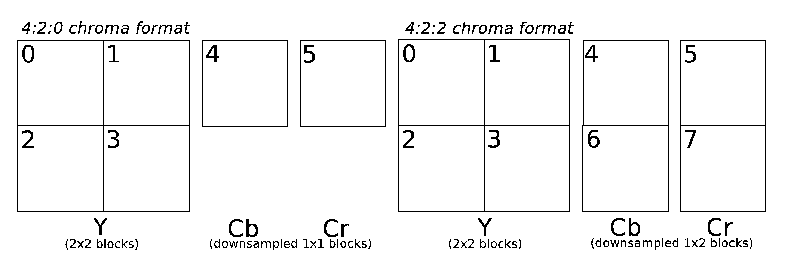
\epsfig{file=chroma_format.eps, width=3in}
    \caption{4:2:0 and 4:2:2 chrominance formats showing macroblock ordering}
    \label{fig:chroma-format}
   \end{center}
  }
  \end{minipage}
\end{figure*}





\SubSection{Motion Compensation}

An MPEG decoder accepts a bitstream as input and performs Huffman and
variable run-length decoding (VLD).  This process results in a set of
quantized, frequency-domain macroblocks and corresponding motion
vectors.  The decoder inverse quantizes (IQ) the macroblocks and then
performs an inverse DCT (IDCT) to convert the macroblocks to the
spatial domain.  For predictively coded macroblocks (e.g., P and B
pictures), the decoder performs motion compensation (MC) using the
input motion vectors to find a corresponding macroblock in a
previously decoded, stored reference picture. This reference
macroblock is added to the current macroblock to recover the original
picture data. If the current macroblock is part of an I or P picture,
then the decoder stores it for future reference.
Figure~\ref{fig:dec_block} illustrates the decode sequence.

\begin{figure}[htbp]
\centerline{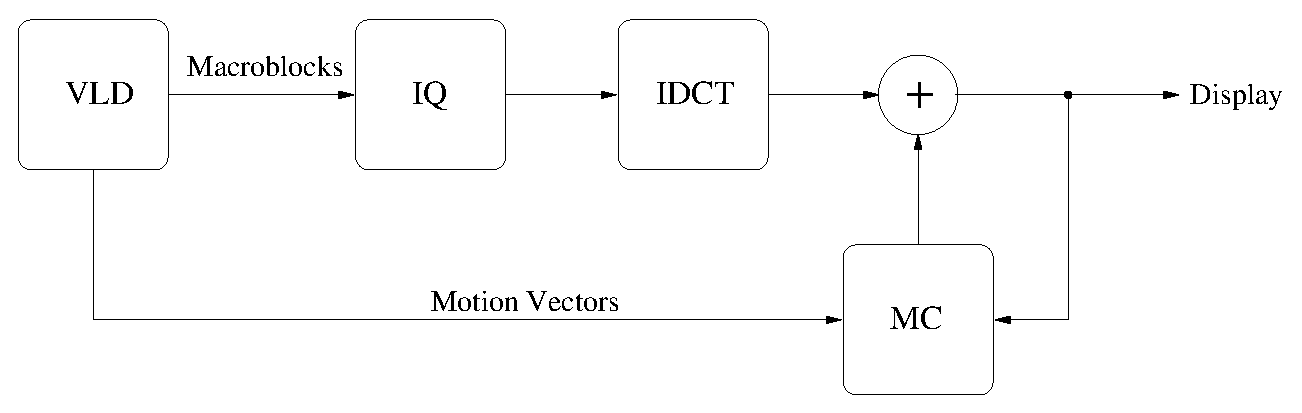
\epsfig{file=dec_block.eps,width=5in}}
\caption{Block diagram of MPEG-2 decode.}
\label{fig:dec_block}
\end{figure}

A simple strategy for parallelizing the MPEG-2 decoding can exploit
the data parallelism among macroblocks. Using this scheme, the Huffman
and run-length decoding is inherently serial, as macroblock boundaries
can only be discovered by performing the decode operation.  Once this
decode is complete, a parallel implementation can distribute
macroblocks to independent streams (using a splitjoin). Each stream
performs the inverse quantization, inverse discrete cosine transform,
and motion compensation. Furthermore, each stream locally stores
reference macroblocks for future motion compensation. Using this
strategy, the streams can execute independently with one exception.

% TODO: This is the figure showing the macroblock parallelism
% I'm not sure where it goes. - Matt
\begin{figure}
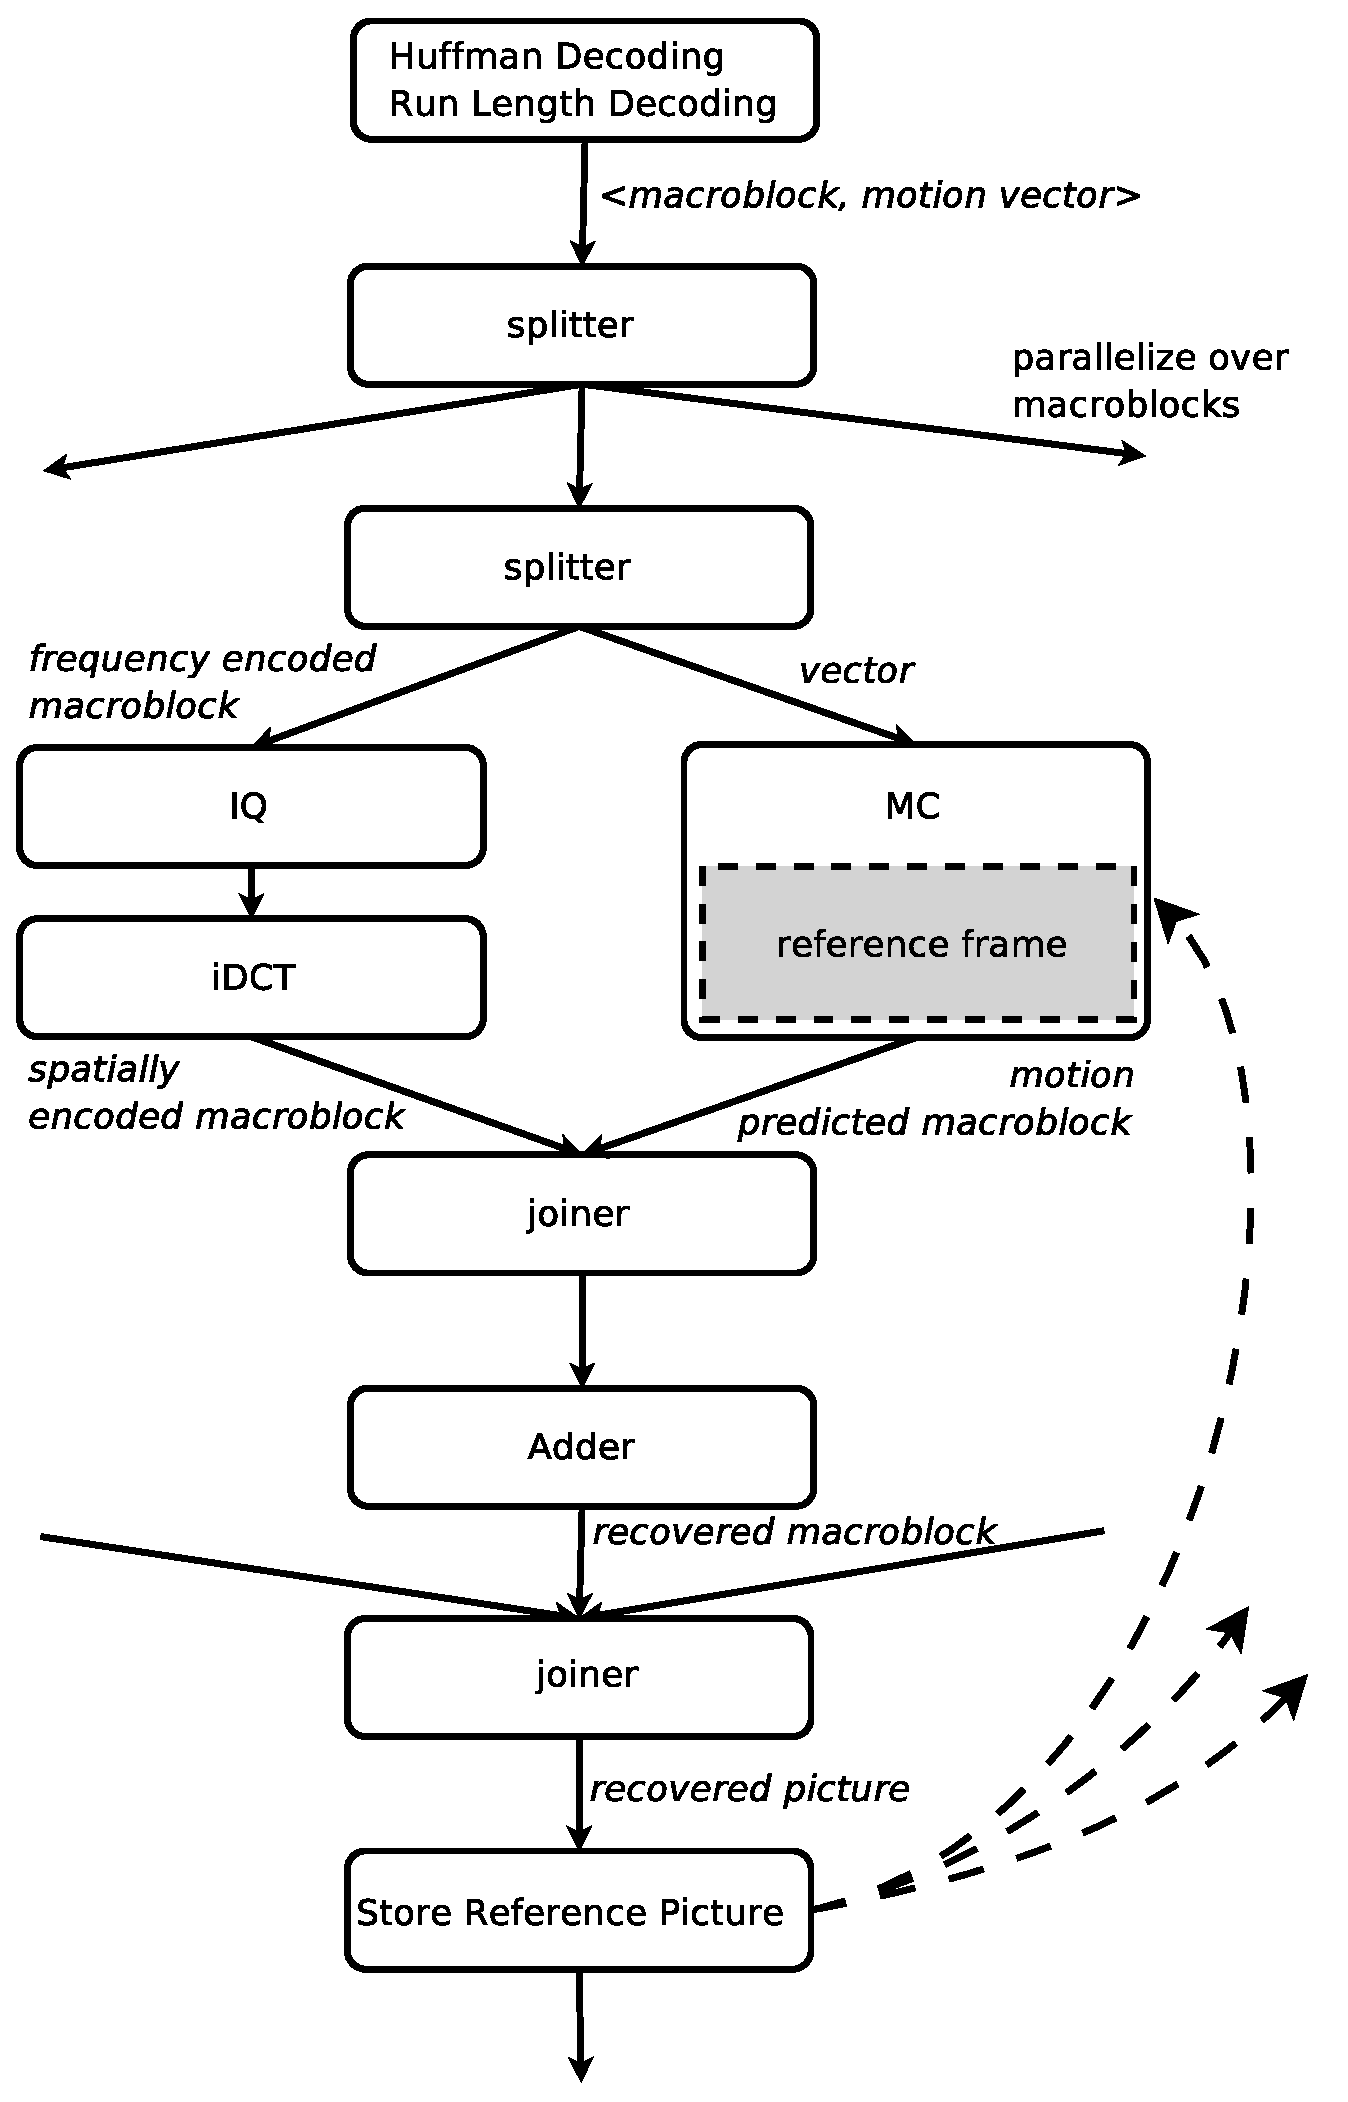
\epsfig{file=decoder_macroblock_parallelism.eps, width=3in}
% TODO: Change Matt's 2 am caption.
\caption{An MPEG-2 Decoder exploiting macroblock parallelism}
\label{decoder_macroblock_parallelism}
\end{figure}

This exception occurs when a stream is performing motion compensation
and the corresponding motion vector indicates a reference macroblock
stored in some other stream. In this case, inter-stream communication
is required to send the reference data to the requesting stream. This
situation is not uncommon, and is more prevalent for higher resolution
pictures. A simple scheme for handling this situation is for every
stream to broadcast its decoded macroblocks to all other streams. This
solution has the benefit of being conceptualy easy to understand and
implement. StreamIt allows programmers to naturally expose such
parallelism. A StreamIt pipeline that operates at macroblock
granularity is shown in Figure~\ref{fig:decoder-macroblock}. It is
worthy to note that there is a high correlation between the stream
graph, and the StreamIt syntax describing the pipeline.

The implementation can be made more fine grained by exposing the
intra-macroblock parallelism. For example, the IQ-IDCT pipeline can
operate at a block level, rather than at a macroblock
granularity. This is easily achieved by encapsulating the IQ-DCT pipeline
within a splitjoin to scatter the blocks, operate, and gather the
results to recover the parent macroblock.

There are many implementation strategies for the decoder, each with
varying degrees of exposed parallelism. Of the greatest advantage of
the StreamIt implemenation is its malleability. The stream graph is
easily reconfigured to operate at picture-level granularity (exposing
parallelism between chroma channels), macroblock level (exposing even
more data-level parallelism), or even at block level (exposing the
greatest amount of data-level parallelism). The modularity of the
language also affords the ability to cleanly define stream interfaces,
and reuse existing components. As an example, the zig-zag descrambler,
inverse quantizer, and inverse DCT components were all reused for our
JPEG codec implementation. The modularity also reduces the complexity
of the debugging process, as stream components can be functionally
verified independently, leading to greater programmer productivity.

%% TODO: add figure showing decoder pipeline at macroblock granularity
%% and streamit text ala Bill's beamformer/fmradio examples


